% -----------------------------------------------------------
% Universidade Federal do Amazonas - UFAM
% Faculdade de Tecnologia - FT
% Engenharia da Computação - FT05
% Período Letivo 2023/01
% -----------------------------------------------------------
% Monografia de Conclusão de Curso entitulada:
% IsenSys - Processador de Solicitações de Isenção de
%           Taxa de Inscrição em Concursos Públicos
% por Felipe André <felipeandre@ufam.edu.br>
% -----------------------------------------------------------
% Utilizando o modelo de pacote 'abntex2', adaptado por
% Roberto Cidade Fonseca, do Instituto de Computação da UFAM,
% disponível em: https://icomp.ufam.edu.br/normas-para-tcc/modelos-de-monografia.html
% -----------------------------------------------------------

\documentclass[
	12pt,			% tamanho da fonte
	openright,		% capítulos começam em página ímpar (insere página vazia caso preciso)
	oneside,	
	a4paper,		% tamanho do papel
	english,		% idioma adicional para hifenização
	brazil			% o último idioma é o principal do documento
]{abntex2/abntex2}  % Entre chaves vai o caminho para o arquivo .cls

% ----------| Pacotes básicos |----------
\usepackage{bookman}			% Usa a fonte 'Bookman Old Style'
\usepackage[T1]{fontenc}		% Seleção de códigos de fonte
\usepackage[utf8]{inputenc}		% Codificação do documento (conversão automática dos acentos)
\usepackage{color}				% Controle das cores
\usepackage{graphicx}			% Inclusão de gráficos
\usepackage{microtype} 			% para melhorias de justificação
\usepackage{indentfirst}        % Indenta o primeiro parágrafo de cada seção.
\usepackage{float}              % Auxilia no posicionamento de imagens

\usepackage[brazilian,hyperpageref]{backref}  % Páginas com as citações na bibl
\usepackage[num]{abntex2cite}                 % Citações no padrão ABNT
\citebrackets[]

% --- 
% CONFIGURAÇÕES DE PACOTES
% --- 

% ---
% Configurações do pacote backref
% Usado sem a opção hyperpageref de backref
\renewcommand{\backrefpagesname}{Citado na(s) página(s):~}
% Texto padrão antes do número das páginas
\renewcommand{\backref}{}
% Define os textos da citação
\renewcommand*{\backrefalt}[4]{
	\ifcase #1 %
	Nenhuma citação no texto.%
	\or
	Citado na página #2.%
	\else
	Citado #1 vezes nas páginas #2.%
	\fi}%
% ---

% ----------| Preâmbulo |----------
\titulo{IsenSys - Processador de Solicitações de Isenção de Taxa de Inscrição em Concursos Públicos}
\tituloeng{IsenSys - A Processor of Public Examination Subscription Fee Requests for Exemption}
\autor{Felipe André Souza da Silva}
\local{Manaus - AM}
\data{Novembro de 2023}
\orientador[Orientador:]{Dr. Edson Nascimento Silva Júnior}
\instituicao{Universidade Federal do Amazonas}
\curso{Bacharelado em Engenharia da Computação}
\tipotrabalho{Monografia}
\preambulo{Monografia de Graduação apresentada à Faculdade de Tecnologia da UFAM como requisito parcial para a obtenção do grau de bacharel em Engenharia da Computação.}

% ----------| Informações do PDF |----------
\makeatletter
\hypersetup{
	pdftitle={\@title}, 
	pdfauthor={\@author},
    pdfsubject={\imprimirpreambulo},
    pdfcreator={LaTeX with abnTeX2},
	pdfkeywords={abnt}{latex}{abntex}{abntex2}{trabalho acadêmico},
	colorlinks=true,
	linkcolor=blue,
	citecolor=black,
	filecolor=magenta,
	urlcolor=blue,
	bookmarksdepth=4
}
\makeatother

% ----------| Espaçamentos entre linhas e parágrafos |----------
\setlength{\parindent}{1.3cm}

% ----------| Compila o Índice |----------
\makeindex

% ----------| Início do Documento |----------
\begin{document}

\noindent

% Seleciona o idioma do documento (conforme pacotes do babel)
\selectlanguage{brazil}

% Retira espaço extra obsoleto entre as frases
\frenchspacing

% Compila a Capa
\imprimircapa

% Compila a Folha de rosto (o * indica que haverá a ficha bibliográfica)
\imprimirfolhaderosto*

% Folha de aprovação
%
% Isto é um exemplo de Folha de aprovação, elemento obrigatório da NBR
% 14724/2011 (seção 4.2.1.3). Você pode utilizar este modelo até a aprovação
% do trabalho. Após isso, substitua todo o conteúdo deste arquivo por uma
% imagem da página assinada pela banca com o comando abaixo:
%
% \includepdf{folhadeaprovacao_final.pdf}
%
\begin{folhadeaprovacao}
	\parindent=0pt
	\setlength{\ABNTEXsignskip}{1.5cm}

	Monografia de Graduação sob o título \textit{\imprimirtitulo} apresentada por {\imprimirautor} e aceita pela Faculdade de Tecnologia da {\imprimirinstituicao}, sendo aprovada por todos os membros da banca examinadora abaixo especificada:

	\assinatura{\fontsize{12}{15}\selectfont {\imprimirorientador} \\ \fontsize{11}{15} \selectfont {\fontsize{10}{12}\selectfont Instituto de Computação \par \imprimirinstituicao }}
	\vspace{1cm}
	\assinatura{Dra. Fabíola Guerra Nakamura \\ {\fontsize{10}{12}\selectfont Instituto de Computação \par \imprimirinstituicao}}
	\vspace{1cm}
	\assinatura{Dr. José Francisco Magalhães Netto \\ {\fontsize{10}{12}\selectfont Instituto de Computação \par \imprimirinstituicao}}
	\vfill
      
	\begin{center}
		\fontsize{12}{15}\selectfont
		\vspace*{0.5cm}
		\imprimirlocal, data de aprovação (por extenso).
		\vspace*{1cm}
	\end{center}
  
\end{folhadeaprovacao}

% Dedicatória
\begin{dedicatoria}
   \vspace*{\fill}
   \noindent
   \leftskip=7cm
   \textit{À minha mãe, mulher guerreira e fonte de inspiração e forças para conclusão deste curso de graduação.}
   \vspace{5cm}
\end{dedicatoria}

% Agradecimentos
\begin{agradecimentos}

Agradecimentos dirigidos àqueles que contribuíram de maneira relevante à elaboração do trabalho, sejam eles pessoas ou mesmo organizações.

\end{agradecimentos}

% Epígrafe
\begin{epigrafe}
    \vspace*{\fill}
	\begin{flushright}
		\textit{Lorem ipsum}

		Autor
	\end{flushright}\vspace{4cm}
\end{epigrafe}

% ---
% RESUMOS
% ---

% resumo em português
\setlength{\absparsep}{18pt} % ajusta o espaçamento dos parágrafos do resumo
\begin{resumo}

	Este documento versa sobre o desenvolvimento de um aplicativo computacional para processar solicitações de isenção de taxa de inscrição em concursos públicos de acordo com as normativas do Ministério do Desenvolvimento Social do Brasil e os interesses da Comissão Permanente de Concursos da UFAM. O sistema, que opera coletivamente com o Sistema de Isenção de Taxa de Concurso, do Ministério do Desenvolvimento Social do Brasil, permite que um órgão gestor prepare dados pessoais de candidatos solicitantes de isenção de taxa de inscrição para envio ao sistema do Ministério do Desenvolvimento, e após o processamento de tais solicitações pelo sistema, gere editais de publicação e relatórios com o objetivo de garantir a lisura e transparência deste processo tão democrático. No desenvolvimento foi utilizada a linguagem de programação \textit{Java} e tecnologias de grande consolidação no mercado como o \textit{Jasper Reports}, para geração de relatórios e o \textit{Apache POI}, adicionando suporte a arquivos do \textit{Microsoft Excel}.

	\vspace{\onelineskip}

	\noindent
	\textit{Palavras-chave}: taxa de inscrição, isenção, concurso público, Java.

\end{resumo}

% resumo em inglês
\begin{abstracteng}[Abstract]
 \begin{otherlanguage*}{english}
 	
 	This document relates to the development of a computer application that facilitates applying for the waiving of fees when sitting public examinations. This is in accordance with the guidelines set by the Brazilian Ministry of Social Development and the requirements of the UFAM Permanent Commission for Examinations. The app system works with the System of Exemption Fees of the Ministry, allowing anyone concerned to handle the personal data of candidates applying for exemption, in order for it to be sent to the Ministry's system. After this process, it creates a public notice and reports, guaranteeing smoothness and transparency in the democratic process. \textit{Java} programming language was used in the development of the app. Other compatible technologies, such as \textit{Jasper Reports}, was used to generate reports and the \textit{Apache POI}, for the processing of \textit{Microsoft Excel} files.

   \vspace{\onelineskip}
 
   \noindent 
   \textit{Keywords}: examination fee, exemption, public examination, Java.
   
 \end{otherlanguage*}
\end{abstracteng}

% ---
% inserir lista de figuras
% ---
\pdfbookmark[0]{\listfigurename}{lof}
\listoffigures*
\cleardoublepage
% ---

% ---
% inserir lista de tabelas
% ---
\pdfbookmark[0]{\listtablename}{lot}
\listoftables*
\cleardoublepage
% ---

% ---
% inserir lista de abreviaturas e siglas
% ---
\begin{siglas}
  \item[COMPEC] Comissão Permanente de Concursos
  \item[MDS] Ministério do Desenvolvimento Social
  \item[NIS] Número de Identificação Social
  \item[PSConcursos] Sistema de Concursos da UFAM
  \item[SISTAC] Sistema de Isenção de Taxa de Concurso
  \item[UFAM] Universidade Federal do Amazonas
\end{siglas}
% ---

% ---
% inserir lista de símbolos
% ---
\begin{simbolos}
  \item[$ \lambda $] Lambda
\end{simbolos}
% ---

% ---
% inserir o sumario
% ---
\pdfbookmark[0]{\contentsname}{toc}
\tableofcontents*
\cleardoublepage
% ---

\textual

\chapter{Introdução}
	
	Com a missão de cultivar o saber em todas as áreas do conhecimento por meio do ensino, pesquisa e da extensão, a Universidade Federal do Amazonas (UFAM) é uma das principais
	portas de entrada para o desenvolvimento pessoal e intelectual, contando com cerca de 29.000 alunos e 3.400 servidores distribuídos em seis \textit{campi} ao redor do Estado do Amazonas, em 2023.
	
	Tomando como objeto de estudo e inspiração para este trabalho, um setor específico desta universidade foi adotado: a Comissão Permanente de Concursos (COMPEC), que é um órgão
	suplementar responsável pela execução dos principais processos seletivos de graduação e concursos para provimento de cargos da universidade.
	
	Uma das tarefas mais democráticas e delicadas executadas por este setor é o processo de isenção de pagamento de taxa de inscrição em concursos e processos seletivos.
	
	Atualmente a COMPEC, como qualquer outra entidade do poder executivo do Brasil, adota três tipos de categorias de isenção: por cadastro no Registro Brasileiro de Doadores Voluntários de Medula Óssea (REDOME), por comprovação de baixa renda e curso de nível médio de forma gratuita e por meio do Cadastro Único para Programas Sociais do Governo Federal (CadÚnico).
	
	Um dos desafios enfrentados pela COMPEC é a gerência e correto processamento das solicitações de isenção, de forma a não prejudicar os candidatos, tampouco a imagem da UFAM e do funcionalismo público. Para ilustrar, apenas em 2023 a COMPEC realizou 10 concursos, mobilizando ao total 39.289 candidatos, onde 8.353 deles tiveram isenção de taxa de inscrição concedida.
	
	Com o intuito de automatizar e otimizar tal processo, este trabalho apresenta uma aplicação de computador capaz de analisar, processar e gerar relatórios e editais de publicação, tomando como objeto de estudo a categoria de isenção mais volumosa em termos de solicitação: a categoria via CadÚnico, regulamentada pelo decreto n{\textdegree} 6.593, de 2 de outubro de 2008.
	
	A aplicação, denominada \textit{IsenSys}, procura ainda fornecer uma interface simples e objetiva, com dicas e tratamentos de forma a instruir intuitivamente sua utilização ao usuário, tomando ainda como alicerce no seu desenvolvimento, os cinco princípios fundamentais da Administração Pública do Brasil: legalidade, impessoalidade, moralidade, publicidade e eficiência.

	\section{Objetivos}
	
		\subsection{Objetivo Geral}
		
		Este projeto possui como objetivo apresentar um aplicativo processador de solicitações de isenção de taxa de inscrição de acordo com a regulamentação do CadÚnico, de forma a permitir agilidade e acurácia nos resultados, por parte de uma unidade gestora do governo federal do Brasil.
		
		\subsection{Objetivos Específicos}
		
		\begin{itemize}
			
			\item Objetivo 1;
			\item Objetivo 2;
			\item Objetivo 3;
			\item Objetivo 4;
			
		\end{itemize}
		
	\section{Organização da Monografia}
	
		Nesta seção deve ser apresentado como está organizado o trabalho, sendo descrito, portanto, do que trata cada capítulo.

\chapter{Referencial Teórico}

	Este capítulo referencia as principais ferramentas utilizadas no desenvolvimento da aplicação \textit{IsenSys}, tais como linguagem de programação e bibliotecas de funções.
	
	\section{Java}
	
	A linguagem de programação Java \cite{java} é uma das mais bem conceituadas e utilizadas ao redor do mundo. Concebida em meados de 1995 pela empresa \textit{Sun Microsystems}, tem conquistado o mundo pela sua simplicidade, forma de organização e versatilidade entre os vários sistemas operacionais.
	
	Por ser uma linguagem independente de plataforma, ela permite que uma mesma aplicação possa ser executada em diversos sistemas operacionais de diversas arquiteturas, sem a necessidade de adaptação ou reconstrução de código por parte do desenvolvedor, comportamento que torna suas aplicações escaláveis e robustas.
	
	\begin{figure}[H]
		
		\caption{\label{java-logo}Logomarca do \textit{Java}}
		\begin{center}
			
\includegraphics[scale=0.04]{img/java-logo}
		\end{center}
		\legend{Fonte: \url{https://www.oracle.com/br/java/technologies/java-se-glance.html}}
		
	\end{figure}
	
	Atualmente mantida pela empresa \textit{Oracle Corporation}, a linguagem continua sendo livre e gratuita para utilização pessoal e para algumas classes de aplicações, e possui uma rica e extensa comunidade de suporte e documentação. As atualizações regulares também são gratuitas e sempre trazem otimizações, novas funcionalidades e melhorias de segurança.

	Provavelmente o leitor já tenha utilizado algumas das aplicações implementadas utilizando a tecnologia Java, tais como os programas de declaração de imposto sobre a renda (IRPF e IRPJ), Processo Judicial Eletrônico (PJe), \textit{MATLAB}, famoso no mundo da engenharia e até o próprio sistema \textit{Android}, um dos principais sistemas operacionais para dispositivos móveis.
	
	\section{JasperReports\textregistered}
	
	A biblioteca \textit{JasperReports\textregistered} \cite{jasper} é gratuita e uma das mais robustas e populares utilizadas para criação de relatórios em \textit{Java}. Possui sua própria suíte de design, onde o desenvolvedor pode rapidamente configurar um novo relatório com poucos passos, seguindo guias e instruções no editor.
	
	Por ser desenvolvida utilizando a linguagem \textit{Java}, ela também apresenta o mesmo comportamento em qualquer sistema operacional onde está disponível, produzindo relatórios de alta qualidade e escalabilidade, oferecendo opções de exportação para outros formatos conhecidos, tais como \textit{PDF}, \textit{Web} e \textit{Microsoft Word}.
	
	\begin{figure}[H]
		\caption{\label{jasper-reports}Suíte de desenvolvimento \textit{JasperReports\textregistered}.}
		\begin{center}
			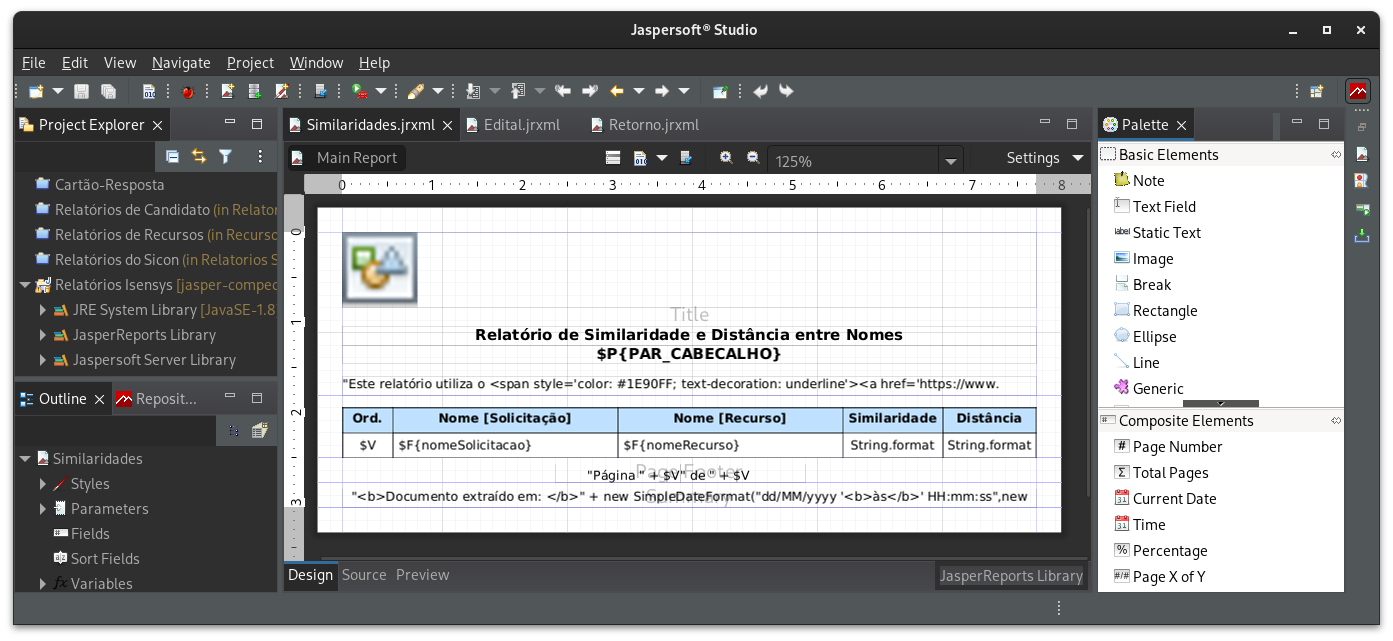
\includegraphics[scale=0.35]{img/jaspersoft}
		\end{center}
		\legend{Fonte: Produzida pelo autor}
	\end{figure}

	\section{Apache POI}
	
	O \textit{Apache POI} \cite{poi} também é uma biblioteca gratuita escrita utilizando a linguagem \textit{Java}, que adiciona suporte de leitura e escrita de dados em documentos do \textit{Microsoft Office} diretamente das aplicações \textit{Java}, sem a necessidade de aquisição e instalação dos aplicativos da \textit{Microsoft}.
	
	Este complemento é desenvolvido e mantido pela \textit{fundação Apache}, que é uma organização mundial sem fins lucrativos criada para dar suporte de desenvolvimento a projetos de programação de código aberto, ou seja, livres para todos.
	
	Por ser uma fundação composta por uma comunidade descentralizada, suas soluções estão em constante melhoria, fornecendo ao desenvolvedor final peças de \textit{software} com qualidade garantida.

	\begin{figure}[H]
		\caption{\label{apache-poi}Logo da biblioteca \textit{Apache POI}.}
		\begin{center}
			
\includegraphics[scale=0.35]{img/apache-poi}
		\end{center}
		\legend{Fonte: \url{https://poi.apache.org}}
	\end{figure}

	\section{Apache Maven}
	
	Até o presente momento foram citadas algumas bibliotecas utilizadas como complemento de código para a linguagem \textit{Java}, prática muito comum entre os desenvolvedores em qualquer linguagem de programação. Porém, muitas vezes sua gerência pode ser complicada se realizada de forma manual, pois bibliotecas resultam em arquivos, que podem sofrer corrompimento ou passar por atualizações de versão.
	
	O \textit{Apache Maven} \cite{maven} surge como uma ferramenta de gerenciamento e compreensão de projetos escritos em \textit{Java}, onde é possível organizar bibliotecas e publicá-las de forma gratuita para utilização pela comunidade de desenvolvimento. Podemos esperar também funcionalidades como atualizações, verificação de integridade e autoinstalação.
	
	A utilização deste gerente é muito simples, tendo em vista que muitas suítes de desenvolvimento oferecem suporte nativo ao \textit{Maven}. Após instalada, basta organizar as dependências (bibliotecas) do projeto em um arquivo especifico denominado 'pom.xml'.

	\begin{figure}[H]
		\caption{\label{maven-logo}Logo do gerente de projetos \textit{Apache Maven}.}
		\begin{center}
			
\includegraphics[scale=0.5]{img/maven-logo}
		\end{center}
		\legend{Fonte: \url{https://maven.apache.org}}
	\end{figure}

	\section{Eclipse IDE}
	
	No mundo do desenvolvimento de software, agilidade e escalabilidade estão entre as qualidades mais requisitadas nas linguagens. Como forma de satisfazer tais demandas, existe no mercado uma vasta gama do que chamamos de \textit{IDE - integrated development environment} ou ambiente de desenvolvimento integrado, amplamente aceitos pela comunidade.
	
	Inicialmente o projeto \textit{Eclipse} \cite{eclipse} foi concebido pensando no desenvolvimento utilizando a linguagem \textit{Java}, mas atualmente suporta extensões \textit{(plugins)} que adicionam suporte a várias outras linguagens, tais como \textit{PHP}, \textit{Python}, \textit{Arduino} etc.
	
	O aplicativo adiciona funcionalidades que auxiliam muito no desenvolvimento em uma linguagem, tais como autocomplemento de código, exibição de sugestões, dicas e tratamentos de erros, verificador de sintaxe e semântica e até integração com outras tecnologias como versionadores de código e até o já mencionado \textit{Apache Maven} \cite{maven}.

	\begin{figure}[H]
		\caption{\label{eclipse-ide}\textit{Eclipse IDE}.}
		\begin{center}
			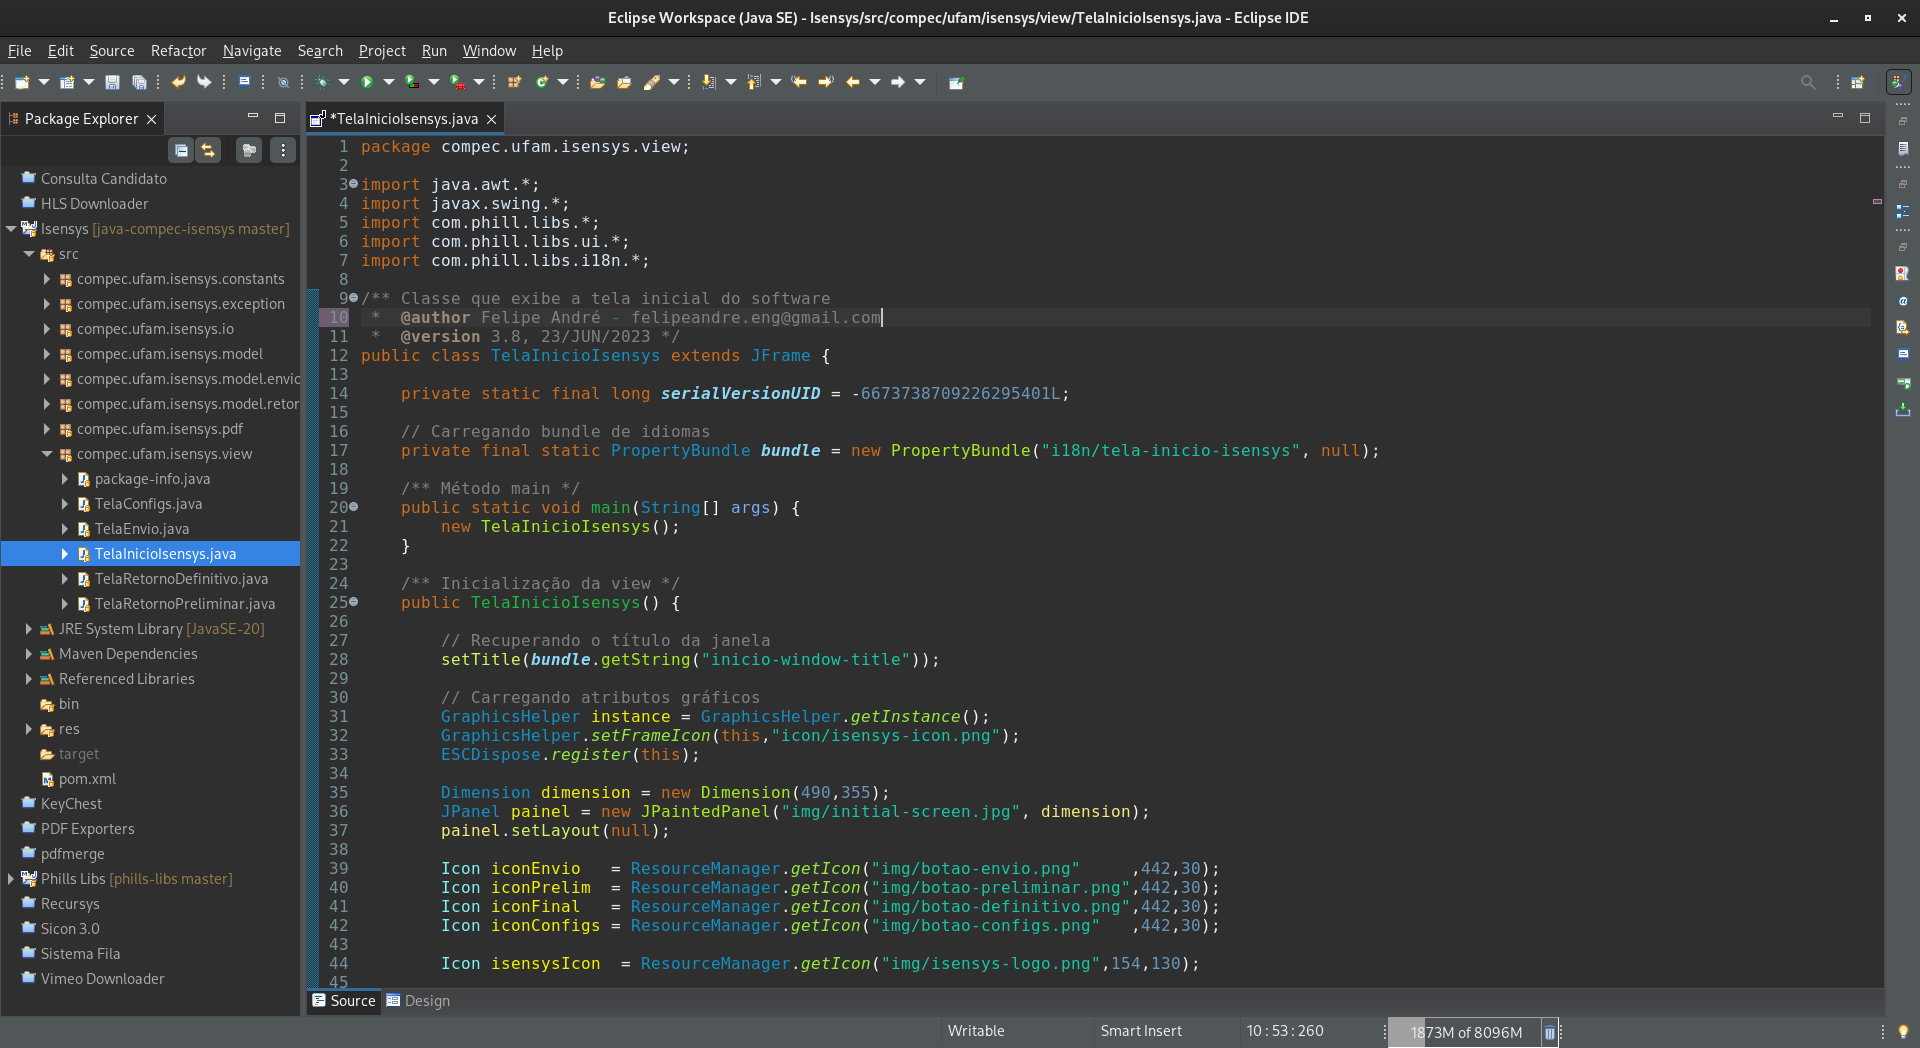
\includegraphics[scale=0.25]{img/eclipse-ide}
		\end{center}
		\legend{Fonte: Produzida pelo autor}
	\end{figure}

\chapter{Desenvolvimento do \textit{IsenSys}}

	Introduzidas as principais ferramentas utilizadas no projeto, aprofundar-se-á no processo de desenvolvimento do aplicativo \textit{IsenSys}. Conceitos como especificações de sistema, requisitos para utilização e formas de aplicação serão demonstrados de forma completa porém, concisa.
	
	O desenvolvimento do \textit{motor} do sistema é regido pelas normas de formato de arquivo e diretivas definidas no documento de orientações gerais do SISTAC \cite{sistac-gerais} e no manual de envio e recebimento de arquivos \cite{sistac-formatos}, versão 10.0, publicada em 24/06/2016.
	
	Os requisitos funcionais (RF) do sistema são:
	
	\begin{itemize}

		\item O sistema deverá permitir a importação de dados de candidatos através de arquivos do tipo \textit{csv} ou planilhas do \textit{Microsoft Excel} (RF01);
		\item O sistema deverá permitir o cadastro e edição de dados da instituição gerente (RF02);
		\item O sistema deverá realizar testes de integridade nos dados importados (RF03);
		\item O sistema deverá gerar arquivos de importação para o SISTAC (RF04);
		\item O sistema só pode entregar um arquivo de importação com os dados de candidatos em sua plena completude e integridade (RF05);
		\item Dados de candidatos que foram informados de forma incompleta ou inválida deverão ser exportados em uma planilha de erros (RF06);
		\item O sistema deverá permitir a importação do arquivo de retorno do SISTAC (RF07);
		\item A partir do arquivo de retorno do SISTAC, o sistema deverá produzir editais de publicação de resultados (RF08);
		\item O sistema também deve permitir a importação de uma planilha com erros, para inclusão nos editais públicos (RF09);
		\item O sistema deve gerar relatórios de estatísticas de candidatos deferidos e indeferidos (RF10);
		\item O sistema deverá gerar um relatório de similaridade entre nomes de candidatos recursantes (RF11).
		
	\end{itemize}
	
	Os requisitos não-funcionais (RF) do sistema são:
	
	\begin{itemize}
		
		\item A linguagem \textit{Java Standard Edittion (Java SE)} foi utilizada no desenvolvimento da aplicação (RNF01);
		\item A versão mínima da \textit{Java Virtual Machine (JVM)} a ser utilizada é a 15 (RNF02);
		\item O projeto foi desenvolvido utilizando o \textit{Java Development Kit (OpenJDK)} na versão 21 (RNF03);
		\item A suíte de interface gráfica utilizada é o \textit{Java Swing} (RNF04);
		\item Por questões de simplicidade, todas as telas foram construídas utilizando layout absoluto com janela não redimensionável (RNF05);
		\item A versão do \textit{Apache POI} utilizada é a 5.2.3, lançada em 17/09/2022 (RNF06);
		\item A versão do \textit{JasperReports\textregistered} utilizada é a 6.26.0, lançada em 11/09/2023 (RNF07);
		\item O sistema pode ser executado em qualquer computador com suporte mínimo à \textit{JDK 15}, mínimo de 1GB de memória RAM disponível e monitor com resolução mínima de 800x600 (RNF08).
		
	\end{itemize}
	
	O sistema conta com dois módulos distintos: um dedicado a preparar os dados de candidatos para envio ao SISTAC e outro dedicado a processar os arquivos de retorno do SISTAC e produzir relatórios e editais de publicação. As seções a seguir contém um estudo mais aprofundado sobre a implementação de cada módulo.

	\section{Desenvolvimento do Módulo de Envio}
	
	Esta seção tem por objetivo detalhar o desenvolvimento do motor \textit{(backend)} de preparação de dados de candidatos para envio ao SISTAC. Primeiramente precisamos entender como está distribuído o fluxo de informações pelo sistema. Para isto, serão detalhadas as entidades principais e auxiliares deste módulo.
	
	\subsection{Modelagem de um Candidato}
	
	Os dados pessoais de um candidato são o objeto principal deste sistema, pois são eles quem solicitam isenção e têm uma resposta de deferimento ou não destas. Segundo o manual do SISTAC \cite{sistac-formatos}, os dados pessoais de candidatos necessários para o processamento estão dispostos na tabela a seguir.

	% Tabela gerada com o auxílio da aplicação: https://www.tablesgenerator.com/latex_tables
	\begin{table}[H]
	
		\caption{Dados pessoais de candidatos e seus formatos.}
		\label{tabela-dados-candidato}
	
		\begin{tabular}{|c|l|c|c|c|}
			\hline
			\textbf{Campo} & \multicolumn{1}{c|}{\textbf{Descrição}} & \textbf{\begin{tabular}[c]{@{}c@{}}Máximo de\\ Caracteres\end{tabular}} & \textbf{Tipo} & \textbf{Formato} \\ \hline
			Nome & \begin{tabular}[c]{@{}l@{}}Nome completo do candidato\\ sem caracteres especiais e\\ sem abreviações\end{tabular} & 100 & Texto &  \\ \hline
			NIS & \begin{tabular}[c]{@{}l@{}}Número de identificação social\\ do candidato\end{tabular} & 11 & Numérico &  \\ \hline
			\begin{tabular}[c]{@{}c@{}}Data de\\ Nascim.\end{tabular} & \begin{tabular}[c]{@{}l@{}}Data de nascimento do\\ candidato\end{tabular} & 8 & Numérico & ddmmaaaa \\ \hline
			Sexo & Sexo do candidato & 1 & Texto & M ou F \\ \hline
			RG & \begin{tabular}[c]{@{}l@{}}Número do Documento de\\ Identidade do candidato\end{tabular} & 16 & \begin{tabular}[c]{@{}c@{}}Alfanu-\\ mérico\end{tabular} &  \\ \hline
			\begin{tabular}[c]{@{}c@{}}Data de\\ Emissão\end{tabular} & \begin{tabular}[c]{@{}l@{}}Data de emissão do Documen-\\ to de Identidade\end{tabular} & 8 & Numérico & ddmmaaaa \\ \hline
			Sigla RG & \begin{tabular}[c]{@{}l@{}}Sigla do órgão emissor do\\ Documento de Identidade\end{tabular} & 30 & \begin{tabular}[c]{@{}c@{}}Alfanu-\\ mérico\end{tabular} &  \\ \hline
			CPF & Número do CPF do candidato & 11 & Numérico &  \\ \hline
			\begin{tabular}[c]{@{}c@{}}Nome\\ da Mãe\end{tabular} & \begin{tabular}[c]{@{}l@{}}Nome completo da mãe do\\ candidato, sem caracteres\\ especiais e sem abreviações\end{tabular} & 100 & Texto &  \\ \hline
		\end{tabular}
		
	\end{table}
	
	De posse dos dados e tipos, foi concebida a modelagem da entidade \textit{Candidato}, de acordo com o diagrama a seguir.

	% Tabela gerada com o auxílio da aplicação: https://www.tablesgenerator.com/latex_tables
	\begin{figure}[H]
		\begin{center}
			
			\caption{Modelagem da entidade \textit{Candidato}}
			\label{candidato-uml}
			
			\begin{tabular}{|l|}
				\hline
				\multicolumn{1}{|c|}{\textbf{Candidato}} \\ \hline
				+nome: String \\
				+nis: String \\
				+dataNascimento: DateTime \\
				+sexo: char \\
				+rg: String \\
				+dataEmissaoRG: DateTime \\
				+orgaoEmissorRG: String \\
				+cpf: String \\
				+nomeMae: String \\ \hline
				\\ \hline
			\end{tabular}
			
		\end{center}
	\end{figure}
	
	De acordo com o diagrama de classe da entidade \textit{Candidato}, nota-se que esta apenas armazena dados. As validações nos campos são garantidas por uma classe intermediária, detalhada na seção seguinte.
	
	\subsection{A classe \textit{CandidatoBuilder}}
	
	Esta classe é responsável por montar um \textit{Candidato} com os dados extraídos de um arquivo de entrada. Durante esse processo ela realiza uma série de validações nos dados, e caso haja pelo menos uma inconsistência, uma exceção com detalhes desta inconsistência é lançada, caso contrário, significa que foi possível construir um objeto respeitando todos os requisitos do SISTAC \cite{sistac-formatos}. Segue o diagrama de classe do \textit{CandidatoBuilder}.
	
	\begin{figure}[H]
		\begin{center}
			
			\caption{Modelagem da entidade \textit{CandidatoBuilder}}
			\label{candidatobuilder-uml}
			
			\begin{tabular}{|l|}
				\hline
				\multicolumn{1}{|c|}{\textbf{CandidatoBuilder}} \\ \hline
				\\ \hline
				+build() \\
				+parseNome() \\
				+parseNIS() \\
				+parseData() \\
				+parseSexo() \\
				+parseRG() \\
				+parseOrgao() \\
				+parseCPF() \\ \hline
			\end{tabular}
		
		\end{center}
	\end{figure}
	
	Os métodos \textit{parse...()}, responsáveis por realizar validações específicas em cada campo de dados de um \textit{Colaborador}, lançam exceções detalhadas para que, posteriormente, tanto o órgão gestor dos dados quanto o candidato possam ter conhecimento de quais campos enviaram fora de formato e se ainda cabe algum recurso.
	
	Para registrar inconsistências em cada um dos campos de dados de um \textit{Candidato}, é utilizada a classe de exceção \textit{FieldParseException} que, por sua vez, é incorporada à classe de exceção \textit{RowParseException}, montada com todas as exceções percebidas pelo método \textit{build()}.

	\subsection{A classe de exceção \textit{FieldParseException}}
	
	Como forma de descentralizar as tratativas de validação de dados de candidatos, a classe de exceção \textit{FieldParseException} é responsável por armazenar informações sobre o motivo de um campo não ter sido validado e qual campo gerou esta exceção. Esta classe apenas estende a superclasse \textit{Exception} e monta uma \textit{String} formatada com o motivo e o nome do campo que não foi validado.

	\subsection{A classe de exceção \textit{RowParseException}}	

	Com o objetivo de concentrar todas as exceções de validação dos campos de dados de um \textit{Candidato}, a classe de exceção \textit{RowParseException} armazena tais exceções em uma lista encadeada e ainda adiciona informações que ajudam a identificar qual foi o candidato que gerou a(s) exceção(ões) e ainda em qual posição do arquivo de entrada ele está.
	
	A seguir é possível visualizar o diagrama de classe de \textit{RowParseException}.
	
	\begin{figure}[H]
		\begin{center}
			
			\caption{Modelagem da entidade \textit{RowParseException}}
			\label{rowparseexception-uml}

			\begin{tabular}{|l|}
				\hline
				\multicolumn{1}{|c|}{\textbf{RowParseException}} \\ \hline
				+linha: int \\
				+nis: String \\
				+cpf: String \\
				+nome: String \\
				+listaExcecoes: List\textless{}FieldParseException\textgreater{} \\ \hline
				+addException() \\
				+hasException() \\
				+getMessage() \\
				+getErrorSummaryArray() \\
				+getErrorSummaryString() \\ \hline
			\end{tabular}
			
		\end{center}
	\end{figure}

	\subsection{A classe \textit{ParseResult}}
	
	Esta classe é responsável por concentrar o resultado da extração de dados do(s) arquivo(s) de entrada em duas listas:
		
	\begin{enumerate}
			
		\item Lista de \textit{Candidato}: onde são armazenados apenas dados de candidatos que passaram com sucesso por todas as validações de campos;
		\item Lista de \textit{RowParseException}: onde são armazenadas a identificação do candidato e o(s) motivos(s) de invalidação de campo(s).
			
	\end{enumerate}
	
	A seguir podemos compreender melhor a classe por meio de seu diagrama.
	
	\begin{figure}[H]
		\begin{center}
			
			\caption{Modelagem da entidade \textit{ParseResult}}
			\label{parseresult-uml}
			
			\begin{tabular}{|l|}
				\hline
				\multicolumn{1}{|c|}{\textbf{ParseResult}} \\ \hline
				+listaCandidatos: List\textless{}Candidato\textgreater{} \\
				+listaExcecoes: List\textless{}RowParseException\textgreater{} \\ \hline
				+addCandidato() \\
				+addExcecao() \\
				+getListaCandidatos() \\
				+getListaExcecoes() \\
				+sortLists() \\ \hline
			\end{tabular}
			
		\end{center}
	\end{figure}
	
	\subsection{Importadores de Dados de Candidato}
	
	O \textit{IsenSys} é capaz de importar dados pessoais de candidatos em dois formatos:
	
	\begin{enumerate}
		
		\item Arquivo \textit{.csv}: que é um arquivo de texto puro (sem formatação), contendo um cabeçalho na sua primeira linha e os dados pessoais requeridos pelo sistema nas outras linhas. O arquivo deve estar codificado em UTF-8, com separador por tabulação, vírgula ou ponto-e-vírgula.
		
		\item Planilha do \textit{Microsoft Excel (.xlsx)}: a planilha deve conter um cabeçalho na primeira linha com os nomes dos campos e nas demais linhas os dados dos candidatos.
		
	\end{enumerate}

	Nos dois casos a ordem da disposição dos dados é extremamente importante para a correta importação. Tanto as colunas do arquivo \textit{csv} quanto as da planilha do \textit{Microsoft Excel} devem respeitar a seguinte ordem:
	
	\begin{enumerate}
		
		\item Nome completo;
		\item NIS;
		\item Data de nascimento;
		\item Sexo;
		\item Número de RG;
		\item Data de emissão do RG;
		\item Órgão emissor do RG;
		\item CPF;
		\item Nome completo da mãe.
		
	\end{enumerate}
	
	Para cada tipo de arquivo foi implementado um importador, contendo as especificidades de tratamento de cada formato. Os dados extraídos pelos importadores são então enviados ao \textit{CandidatoBuilder} que irá construir um objeto \textit{Candidato}, tornando todo o processo de tratativa de arquivos transparente às classes superiores.
	
	\subsubsection{O importador \textit{CSVSheetReader}}
	
	Para o arquivo \textit{.csv} temos o importador descrito na classe \textit{CSVSheetReader}, que é util tanto para o módulo de envio, através do método \textit{read()}, quanto pelo módulo de retorno, através do método \textit{readRetorno()}. A princípio o papel deste importador é detectar o tipo de separador do arquivo \textit{.csv} e extrair os dados de uma linha. A seguir temos seu diagrama de classe.
	
	\begin{figure}[H]
		\begin{center}
			
			\caption{Modelagem do importador de dados \textit{CSVSheetReader}}
			\label{csvreader-uml}
			
			\begin{tabular}{|l|}
				\hline
				\multicolumn{1}{|c|}{\textbf{CSVSheetReader}} \\ \hline
				\\ \hline
				+read() \\
				+readRetorno() \\
				+readLine() \\
				+getInstituicao() \\ \hline
			\end{tabular}
			
		\end{center}
	\end{figure}
	
	\subsubsection{O importador \textit{ExcelSheetReader}}

	Este importador também é comum aos dois módulos do sistema, mas em momentos distintos. Sua função no módulo de envio é iterar sobre as linhas e colunas de uma planilha com os dados de candidatos e entregá-los ao \textit{CandidatoBuilder}. Seu diagrama de classe está disposto na figura a seguir.

	\begin{figure}[H]
		\begin{center}
			
			\caption{Modelagem do importador de dados \textit{ExcelSheetReader}}
			\label{excelreader-uml}
			
			\begin{tabular}{|l|}
				\hline
				\multicolumn{1}{|c|}{\textbf{ExcelSheetReader}} \\ \hline
				\\ \hline
				+read() \\
				+readErros() \\
				+readLine() \\
				+getCellContent() \\ \hline
			\end{tabular}
			
		\end{center}
	\end{figure}
	
	\subsection{Integração do Módulo de Envio}
	
	Após conhecer individualmente todos os agentes envolvidos no módulo de envio, far-se-á uma análise em conjunto de todos eles, possibilitando compreender o fluxo das informações e os estágios do processo de preparação dos dados dos candidatos para envio ao SISTAC.
	
	\subsection{Interface Gráfica do Módulo de Envio}
	
	

% ----------------------------------------------------------
% ELEMENTOS PÓS-TEXTUAIS
% ----------------------------------------------------------
\postextual
\Spacing{1.5}
% -----------------------------------------------------------------------------
% Referencias Bibliograficas
% -----------------------------------------------------------------------------
\bibliography{monografia-felipe-andre-ft}

% ----------------------------------------------------------
% Apêndices
% ----------------------------------------------------------

% ---
% Inicia os apêndices
% ---
\begin{apendicesenv}

% ----------------------------------------------------------
\chapter{Primeiro apêndice}
% ----------------------------------------------------------

Os apêndices são textos ou documentos elaborados pelo autor, a fim de complementar sua argumentação, sem prejuízo da unidade nuclear do trabalho.

\end{apendicesenv}

% Anexos
% ----------------------------------------------------------

% ---
% Inicia os anexos
% ---
\begin{anexosenv}

% ---
\chapter{Primeiro anexo.}
% ---

Os anexos são textos ou documentos não elaborados pelo autor, que servem de fundamentação, comprovação e ilustração.

\end{anexosenv}

\end{document}